\documentclass[14pt]{extbook}
\usepackage{multicol, enumerate, enumitem, hyperref, color, soul, setspace, parskip, fancyhdr} %General Packages
\usepackage{amssymb, amsthm, amsmath, latexsym, units, mathtools} %Math Packages
\everymath{\displaystyle} %All math in Display Style
% Packages with additional options
\usepackage[headsep=0.5cm,headheight=12pt, left=1 in,right= 1 in,top= 1 in,bottom= 1 in]{geometry}
\usepackage[usenames,dvipsnames]{xcolor}
\usepackage{dashrule}  % Package to use the command below to create lines between items
\newcommand{\litem}[1]{\item#1\hspace*{-1cm}\rule{\textwidth}{0.4pt}}
\pagestyle{fancy}
\lhead{Progress Quiz 6}
\chead{}
\rhead{Version B}
\lfoot{1430-1829}
\cfoot{}
\rfoot{test}
\begin{document}

\begin{enumerate}
\litem{
Determine the domain of the function below.\[ f(x) = \frac{3}{15x^{2} -12 x -36} \]\begin{enumerate}[label=\Alph*.]
\item \( \text{All Real numbers except } x = a, \text{ where } a \in [-3.2, 0.8] \)
\item \( \text{All Real numbers except } x = a, \text{ where } a \in [-32, -28] \)
\item \( \text{All Real numbers.} \)
\item \( \text{All Real numbers except } x = a \text{ and } x = b, \text{ where } a \in [-32, -28] \text{ and } b \in [17, 19] \)
\item \( \text{All Real numbers except } x = a \text{ and } x = b, \text{ where } a \in [-3.2, 0.8] \text{ and } b \in [2, 5] \)

\end{enumerate} }
\litem{
Solve the rational equation below. Then, choose the interval(s) that the solution(s) belongs to.\[ \frac{-2}{-7x + 2} + 3 = \frac{-4}{28x -8} \]\begin{enumerate}[label=\Alph*.]
\item \( \text{All solutions lead to invalid or complex values in the equation.} \)
\item \( x \in [-0.6,-0.2] \)
\item \( x_1 \in [-0.1, 1.3] \text{ and } x_2 \in [0.37,0.53] \)
\item \( x \in [0.14,3.14] \)
\item \( x_1 \in [-0.6, -0.2] \text{ and } x_2 \in [0.1,0.23] \)

\end{enumerate} }
\litem{
Solve the rational equation below. Then, choose the interval(s) that the solution(s) belongs to.\[ \frac{-3x + 0}{-5x + 6} + \frac{-2x^{2} +0 x + 0}{-10x^{2} +22 x -12} = \frac{7}{2x -2} \]\begin{enumerate}[label=\Alph*.]
\item \( x \in [3.58,4.52] \)
\item \( x_1 \in [1.34, 2.52] \text{ and } x_2 \in [1.5,4] \)
\item \( \text{All solutions lead to invalid or complex values in the equation.} \)
\item \( x \in [0.37,1.36] \)
\item \( x_1 \in [1.34, 2.52] \text{ and } x_2 \in [-1.7,2.1] \)

\end{enumerate} }
\litem{
Determine the domain of the function below.\[ f(x) = \frac{3}{30x^{2} -43 x + 15} \]\begin{enumerate}[label=\Alph*.]
\item \( \text{All Real numbers except } x = a, \text{ where } a \in [14.7, 15.08] \)
\item \( \text{All Real numbers except } x = a \text{ and } x = b, \text{ where } a \in [0.1, 0.79] \text{ and } b \in [0.67, 1.24] \)
\item \( \text{All Real numbers except } x = a, \text{ where } a \in [0.1, 0.79] \)
\item \( \text{All Real numbers.} \)
\item \( \text{All Real numbers except } x = a \text{ and } x = b, \text{ where } a \in [14.7, 15.08] \text{ and } b \in [29.71, 30.12] \)

\end{enumerate} }
\litem{
Choose the equation of the function graphed below.
\begin{center}
    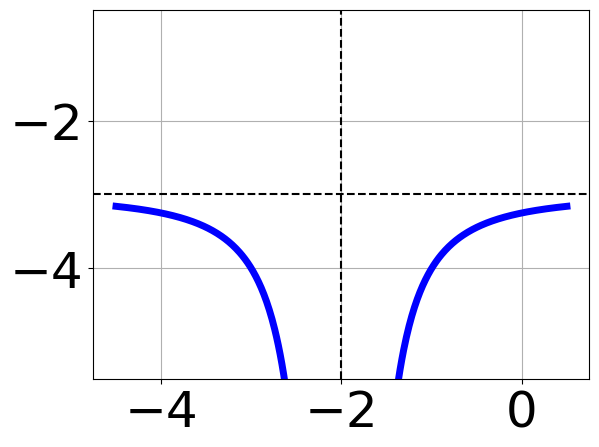
\includegraphics[width=0.5\textwidth]{../Figures/rationalGraphToEquationCopyB.png}
\end{center}
\begin{enumerate}[label=\Alph*.]
\item \( f(x) = \frac{1}{x + 3} - 3 \)
\item \( f(x) = \frac{-1}{(x - 3)^2} - 3 \)
\item \( f(x) = \frac{1}{(x + 3)^2} - 3 \)
\item \( f(x) = \frac{-1}{x - 3} - 3 \)
\item \( \text{None of the above} \)

\end{enumerate} }
\litem{
Choose the graph of the equation below.\[ f(x) = \frac{1}{(x + 3)^2} - 3 \]\begin{enumerate}[label=\Alph*.]
\begin{multicols}{2}\item 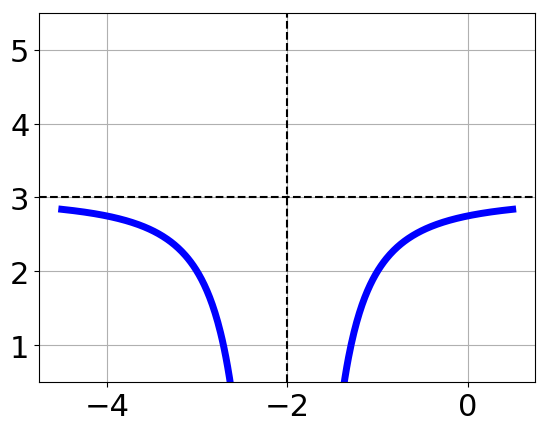
\includegraphics[width = 0.3\textwidth]{../Figures/rationalEquationToGraphAB.png}\item 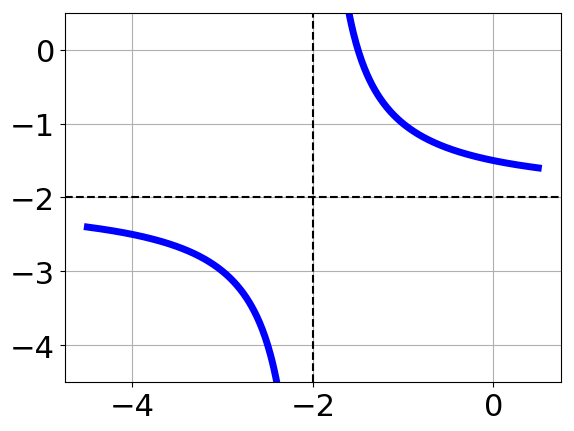
\includegraphics[width = 0.3\textwidth]{../Figures/rationalEquationToGraphBB.png}\item 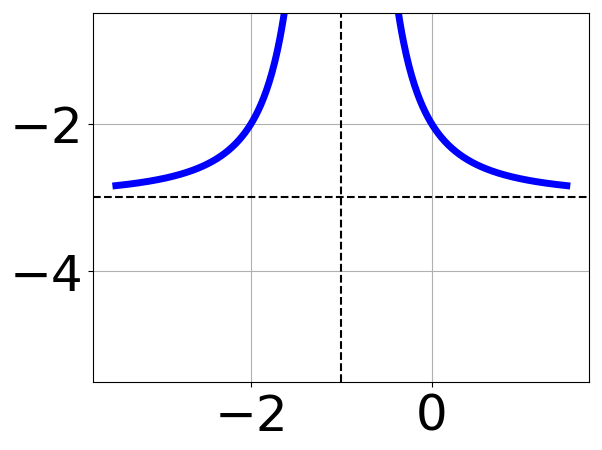
\includegraphics[width = 0.3\textwidth]{../Figures/rationalEquationToGraphCB.png}\item 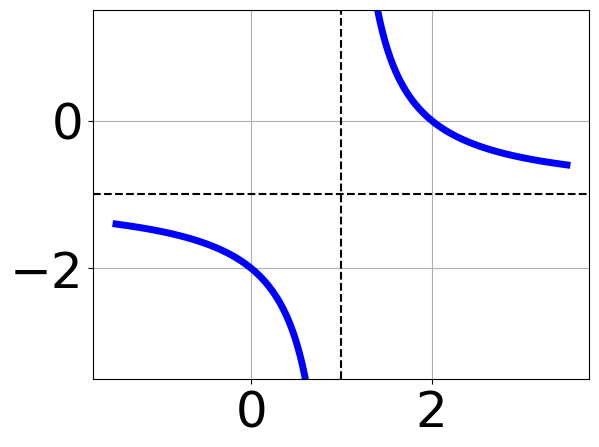
\includegraphics[width = 0.3\textwidth]{../Figures/rationalEquationToGraphDB.png}\end{multicols}\item None of the above.
\end{enumerate} }
\litem{
Solve the rational equation below. Then, choose the interval(s) that the solution(s) belongs to.\[ \frac{-27}{-45x -81} + 1 = \frac{-27}{-45x -81} \]\begin{enumerate}[label=\Alph*.]
\item \( x_1 \in [-4.8, -0.8] \text{ and } x_2 \in [-4.8,-0.8] \)
\item \( x_1 \in [-4.8, -0.8] \text{ and } x_2 \in [0.8,2.8] \)
\item \( x \in [-2.8,-0.8] \)
\item \( \text{All solutions lead to invalid or complex values in the equation.} \)
\item \( x \in [1.8,3.8] \)

\end{enumerate} }
\litem{
Choose the graph of the equation below.\[ f(x) = \frac{-1}{x + 3} + 1 \]\begin{enumerate}[label=\Alph*.]
\begin{multicols}{2}\item 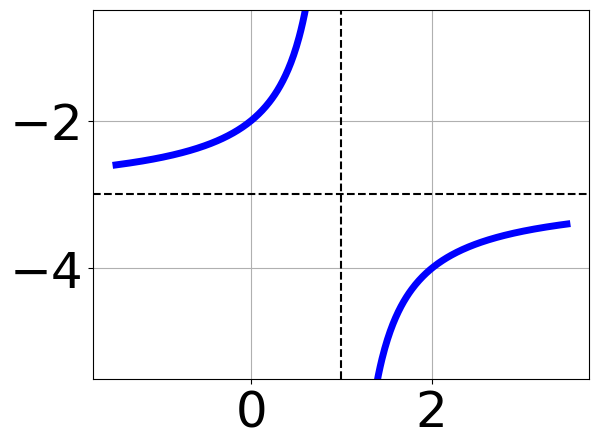
\includegraphics[width = 0.3\textwidth]{../Figures/rationalEquationToGraphCopyAB.png}\item 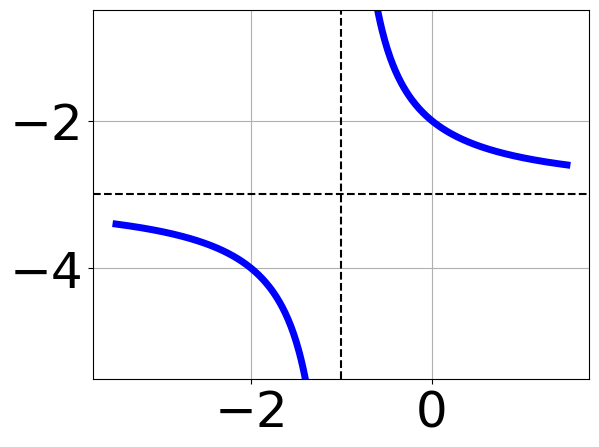
\includegraphics[width = 0.3\textwidth]{../Figures/rationalEquationToGraphCopyBB.png}\item 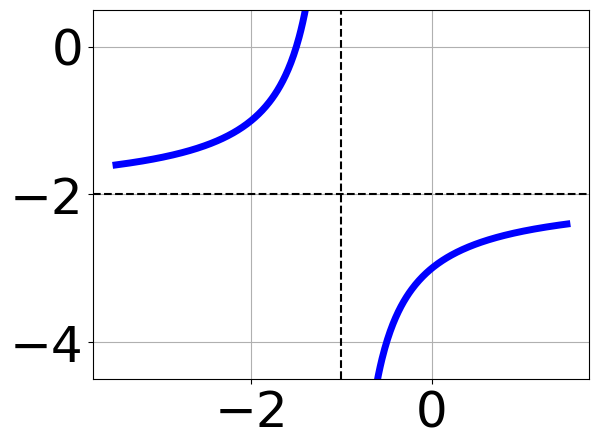
\includegraphics[width = 0.3\textwidth]{../Figures/rationalEquationToGraphCopyCB.png}\item 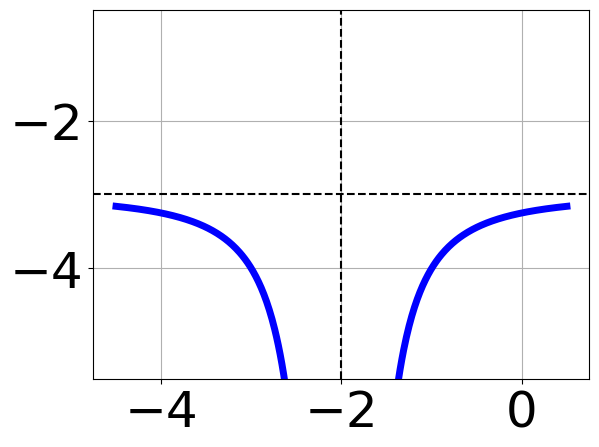
\includegraphics[width = 0.3\textwidth]{../Figures/rationalEquationToGraphCopyDB.png}\end{multicols}\item None of the above.
\end{enumerate} }
\litem{
Choose the equation of the function graphed below.
\begin{center}
    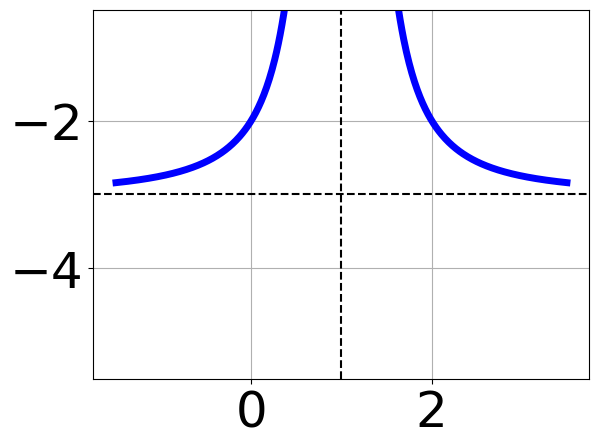
\includegraphics[width=0.5\textwidth]{../Figures/rationalGraphToEquationB.png}
\end{center}
\begin{enumerate}[label=\Alph*.]
\item \( f(x) = \frac{1}{x - 3} - 3 \)
\item \( f(x) = \frac{-1}{x + 3} - 3 \)
\item \( f(x) = \frac{1}{(x - 3)^2} - 3 \)
\item \( f(x) = \frac{-1}{(x + 3)^2} - 3 \)
\item \( \text{None of the above} \)

\end{enumerate} }
\litem{
Solve the rational equation below. Then, choose the interval(s) that the solution(s) belongs to.\[ \frac{4x + 0}{7x + 2} + \frac{-5x^{2} +0 x + 0}{42x^{2} +26 x + 4} = \frac{2}{6x + 2} \]\begin{enumerate}[label=\Alph*.]
\item \( x \in [-0.34,-0.33] \)
\item \( x_1 \in [-0.33, -0.32] \text{ and } x_2 \in [-0.59,0.1] \)
\item \( x \in [0.64,0.65] \)
\item \( \text{All solutions lead to invalid or complex values in the equation.} \)
\item \( x_1 \in [-0.33, -0.32] \text{ and } x_2 \in [0.36,1.05] \)

\end{enumerate} }
\end{enumerate}

\end{document}